\documentclass[11pt,a4paper]{article}
\usepackage[T1]{fontenc}
\usepackage[utf8]{inputenc}
\usepackage{lmodern}
\usepackage[margin=1in]{geometry}
\usepackage{amsmath,amssymb,amsthm,mathtools}
\usepackage{booktabs}
\usepackage{graphicx}
\usepackage{microtype}
\usepackage{xcolor}
\usepackage[colorlinks=true,linkcolor=blue!50!black,citecolor=blue!50!black,urlcolor=blue!50!black]{hyperref}

\newtheorem{theorem}{Theorem}
\newtheorem{proposition}[theorem]{Proposition}
\newtheorem{lemma}[theorem]{Lemma}
\newtheorem{corollary}[theorem]{Corollary}
\theoremstyle{remark}
\newtheorem{remark}[theorem]{Remark}

\newcommand{\ket}[1]{\lvert #1\rangle}
\newcommand{\bra}[1]{\langle #1\rvert}
\newcommand{\ketbra}[2]{\lvert #1\rangle\langle #2\rvert}
\newcommand{\id}{\mathbf{1}}
\newcommand{\tr}{\operatorname{Tr}}
\newcommand{\G}{\Gamma}
\newcommand{\uW}{u_W}
\newcommand{\lmax}{\lambda_{\max}}
% ---- Zenodo archive: put the DOI between the braces once it has been assigned -------------
\def\zenodoDOI{10.5281/zenodo.24442820}
\def\zenodonote{\ifx\zenodoDOI\empty\else\noindent An archived snapshot is available at
Zenodo, \href{https://doi.org/\zenodoDOI}{doi:\zenodoDOI}.\fi}
% -------------------------------------------------------------------------------------------

\hypersetup{pdftitle={Exact separable bounds for covariant entanglement witnesses in every dimension and the absence of non-decomposable mirrors},
  pdfauthor={Ruqing Chen}}

\title{Exact separable bounds for covariant entanglement witnesses\\
in every dimension and the absence of non-decomposable mirrors,\\
with a correction to Quantum Sci.\ Technol.\ 11, 015037 (2026)}
\author{Ruqing Chen\\[2pt]
\small Independent Researcher, Montreal, Quebec, Canada\\
\small \href{mailto:ruqing@hotmail.com}{ruqing@hotmail.com}\quad
ORCID: \href{https://orcid.org/0009-0009-4622-6615}{0009-0009-4622-6615}}
\date{November 17, 2026}

\begin{document}
\maketitle

\begin{abstract}
A mirrored entanglement witness is obtained from a witness $W$ by reflection at its
separable upper bound, $M=\uW\id-W$ with $\uW=\max_{\sigma\ \mathrm{separable}}\tr(W\sigma)$.
We determine $\uW$ exactly for the family of circulant, diagonally covariant operators
$W_\alpha=\sum_{i,k}\alpha_k\ketbra{i,i+k}{i,i+k}-\sum_{i\neq j}\ketbra{ii}{jj}$ on
$\mathbb{C}^n\otimes\mathbb{C}^n$, for every dimension $n$ and all real parameters:
$\uW$ is the largest of the numbers $\alpha_0,\dots,\alpha_{n-1}$ and
$((\alpha_0+1)^2-\alpha_k\alpha_{n-k})/(2(\alpha_0+1)-\alpha_k-\alpha_{n-k})$,
$1\le k\le n/2$, and it is attained on product vectors supported on two levels. The upper
bound is proved by an explicit decomposition $\uW\id-W_\alpha=P+Q^{\G}$ with $P,Q\ge0$.
As a consequence, $\mu\id-W_\alpha$ is block positive if and only if it is decomposable:
in no dimension does a witness of this family have a non-decomposable mirror. This
confirms, for the whole family and without any optimality assumption, the behaviour that
was conjectured for mirrors of optimal witnesses and is known to fail outside the family.
We apply the result to a recent paper of Seong, Bera, Hiesmayr, Chru\'sci\'nski and Bae,
where the mirrored operator of the $4\otimes4$ witness $W[1,1,1,0]$ is given as
$\tfrac43\id-W[1,1,1,0]$ and is stated to be a non-decomposable witness. This operator is
not an entanglement witness: its expectation value on the product vector
$\tfrac12(\ket0+\ket2)\otimes(\ket0-\ket2)$ is $-1/6$. The correct constant is $3/2$, the
corrected mirror is decomposable, and the PPT states proposed there are not detected.
The value $4/3$ is the separable bound of the three-dimensional Choi witness; for the
analogous witness $W[1,\dots,1,0]$ the bound is $3/2$ in every dimension $n\ge4$. We give
a non-decomposable mirrored pair in every $n\otimes n$, $n\ge3$, by an embedding
construction, and report a recomputation of the other explicit examples of the audited
paper.
\end{abstract}

\section{Introduction}

Entanglement witnesses are observables $W$ with $\tr(W\sigma)\ge0$ for all separable
states $\sigma$ and $\tr(W\rho)<0$ for some entangled state
$\rho$~\cite{HHH96,Terhal00,LKCH00,GT09,CS14}. Bae, Chru\'sci\'nski and
Hiesmayr~\cite{BCH20} observed that a witness also has a non-trivial \emph{upper} bound on
separable states,
\begin{equation}\label{eq:uW}
0\le\tr(W\sigma)\le\uW,\qquad \uW=\max_{\sigma\ \mathrm{separable}}\tr(W\sigma)
=\max_{\ket e,\ket f}\bra{e,f}W\ket{e,f},
\end{equation}
and that the reflected operator $M=\uW\id-W$ is then non-negative on separable states.
If $M$ is not positive semidefinite, it is a second witness, the \emph{mirrored} witness,
and it detects a set of entangled states disjoint from the one detected by $W$ at no
additional experimental cost.

A central question is how good a mirror can be: can both members of a mirrored pair be
non-decomposable, that is, able to detect entangled states with positive partial transpose
(PPT)~\cite{Peres96,HHH96}? On the basis of many examples, Bera, Bae, Hiesmayr and
Chru\'sci\'nski~\cite{BBHC23} conjectured that the mirrored operator of an optimal witness
is either positive or a decomposable witness. A mirrored pair of optimal non-decomposable
witnesses in $3\otimes3$ was later found by Chru\'sci\'nski, Bera, Bae and
Hiesmayr~\cite{CBBH25}, so the conjecture does not hold in general. Which families of
witnesses do obey it has remained open.

Seong, Bera, Hiesmayr, Chru\'sci\'nski and Bae~\cite{SBHCB26} (SBHCB in what follows)
develop mirrored witnesses for multipartite and for high-dimensional bipartite systems.
Equation numbers of the form ``SBHCB~(n)'' refer to the arXiv version
\texttt{2510.06863v2} of~\cite{SBHCB26}; that version is dated 16 January 2026, four days
after the publication of the journal article, and we have not compared it line by line
with the version of record. In Section~IV.B of~\cite{SBHCB26} the authors consider the
$4\otimes4$ witnesses
\begin{equation}\label{eq:W4}
W[a,b,c,d]=\sum_{i=0}^{3}\sum_{k=0}^{3}\alpha_k\ketbra{i,i+k}{i,i+k}-\sum_{i\neq j}\ketbra{ii}{jj},
\qquad (\alpha_0,\alpha_1,\alpha_2,\alpha_3)=(a,b,c,d),
\end{equation}
with indices modulo $4$ (SBHCB~(72)), and state for $W[1,1,1,0]$ that the mirrored operator
is
\begin{equation}\label{eq:M43}
M[1,1,1,0]=\tfrac43\,\id_4\otimes\id_4-W[1,1,1,0],
\end{equation}
that it detects the PPT states $\rho_x$ of SBHCB~(75) for $x\in(1,4)$, and hence that
``the mirrored operator $M[1,1,1,0]$ is a non-decomposable EW. We have shown that a pair of
non-decomposable EWs can be mirrored with each other.''

In this paper we solve the separable-bound problem for the natural $n$-dimensional family
that contains \eqref{eq:W4}, and we use the solution to correct the statement above. Our
results are the following.
\begin{enumerate}
\item \emph{Exact separable bound in every dimension}
(Theorems~\ref{thm:cert} and~\ref{thm:exact}). For all $n\ge2$ and all real parameters
we compute $\uW$ in closed form, exhibit the product vectors that attain it, and prove
the upper bound by an explicit decomposition of $\uW\id-W$ into a positive operator and
the partial transpose of a positive operator.
\item \emph{No non-decomposable mirror} (Corollary~\ref{cor:nogo}). For every real $\mu$,
the operator $\mu\id-W_\alpha$ is block positive if and only if it is decomposable. A
mirrored operator of a witness of this family is a decomposable witness or a positive
operator, in every dimension and whether or not the witness is optimal.
\item \emph{Counterexample to the $4\otimes4$ example of SBHCB}
(Section~\ref{sec:counter}). On the product vector
$\tfrac12(\ket0+\ket2)\otimes(\ket0-\ket2)$ one finds
$\langle W[1,1,1,0]\rangle=3/2>4/3$, so the operator \eqref{eq:M43} has the expectation
value $-1/6$ on a separable state.
\item \emph{The two classes of SBHCB} (Section~\ref{sec:classes}). For every member of
class~I, which contains $W[1,1,1,0]$, one has $\uW=3/2$; for class~II, $\uW=3/2$ or
$\uW=\lmax(W)$. With the correct constant the states $\rho_x$ are not detected.
\item \emph{Existence outside the family} (Proposition~\ref{prop:embed}). An embedding
construction turns a non-decomposable mirrored pair in $3\otimes3$ into one in every
$n\otimes n$, $n\ge4$.
\item \emph{Recomputation of the other examples of SBHCB} (Section~\ref{sec:sweep} and
Appendix~\ref{app:pauli}).
\end{enumerate}
The logical structure is short: Lemma~\ref{lem:prod} gives the expectation value on
product vectors, Theorem~\ref{thm:cert} is the decomposition certificate,
Theorem~\ref{thm:exact} combines the two into the exact bound, and
Corollary~\ref{cor:nogo} is the resulting no-go statement.

All theorems are proved analytically. Every formula and number below is in addition
reproduced by the script \texttt{verify\_mirrored\_witnesses.py} that accompanies this
paper; it performs 83 checks, the decisive ones in exact rational or symbolic arithmetic.
Numerical optimization over product vectors is used only as an independent test of the
closed forms and for statements explicitly marked as numerical.

\section{Setting}\label{sec:setting}

Let $n\ge2$ and let $\ket{i,j}=\ket i\otimes\ket j$ be the product basis of
$\mathbb{C}^n\otimes\mathbb{C}^n$, with all indices taken modulo $n$. For a real vector
$\alpha=(\alpha_0,\dots,\alpha_{n-1})$ put
\begin{equation}\label{eq:Walpha}
W_\alpha=\sum_{i,k}\alpha_k\ketbra{i,i+k}{i,i+k}-\sum_{i\neq j}\ketbra{ii}{jj}
=D_\alpha+\sum_i\ketbra{ii}{ii}-n\ketbra{\phi^+}{\phi^+},
\end{equation}
where $D_\alpha$ is the diagonal part and $\ket{\phi^+}=n^{-1/2}\sum_i\ket{ii}$. These are
the operators of SBHCB~(68); they are covariant under $U\otimes U^{*}$ for diagonal
unitaries $U$ and invariant under the simultaneous cyclic shift of both labels. For $n=3$
we write $W[a,b,c]$ (SBHCB~(70)) and for $n=4$ we write $W[a,b,c,d]$ as in
\eqref{eq:W4}. The spectrum is read off from \eqref{eq:Walpha}: $\alpha_0+1-n$ on
$\ket{\phi^+}$, $\alpha_0+1$ on the rest of $\operatorname{span}\{\ket{ii}\}$, and
$\alpha_k$ on $\ket{i,i+k}$, $k\neq0$. In particular
\begin{equation}\label{eq:lmax}
\lmax(W_\alpha)=\max\{\alpha_0+1,\alpha_1,\dots,\alpha_{n-1}\}.
\end{equation}

An operator $X$ is \emph{block positive} if $\bra{e,f}X\ket{e,f}\ge0$ for all product
vectors, and \emph{decomposable} if $X=P+Q^{\G}$ with $P,Q\ge0$, where $\G$ denotes the
partial transpose on the first factor. Decomposable operators are block positive and are
non-negative on all PPT states, so they detect no PPT entangled state. A witness is a
block-positive operator that is not positive semidefinite.

For an arbitrary Hermitian operator $W$ we define $\uW$ as the maximum of
$\bra{e,f}W\ket{e,f}$ over unit product vectors, as on the right of \eqref{eq:uW}; no
assumption on $W$ is needed, and for a witness this is the separable upper bound. For a
real number $\mu$ we call $\mu\id-W$ the mirrored operator of $W$ with constant $\mu$; it
is block positive if and only if $\mu\ge\uW$.

\begin{lemma}\label{lem:prod}
For unit vectors $e,f\in\mathbb{C}^n$ let $s_k=\sum_i|e_i|^2|f_{i+k}|^2$. Then
$\sum_ks_k=1$ and
\begin{equation}\label{eq:prodval}
\bra{e,f}W_\alpha\ket{e,f}=\sum_{k=0}^{n-1}\alpha_ks_k+s_0-\Bigl|\sum_ie_if_i\Bigr|^{2}.
\end{equation}
\end{lemma}
\begin{proof}
The diagonal part gives $\sum_k\alpha_ks_k$. For complex $e,f$ one has
$\bra{e,f}ii\rangle\langle jj\ket{e,f}=\overline{e_if_i}\,e_jf_j$, and
$\sum_{i\neq j}\overline{e_if_i}\,e_jf_j=|\sum_ie_if_i|^2-\sum_i|e_if_i|^2$ with
$\sum_i|e_if_i|^2=s_0$.
\end{proof}

\section{The counterexample}\label{sec:counter}

Take $n=4$, $\alpha=(1,1,1,0)$ and
\begin{equation}\label{eq:psistar}
\ket{e}=\frac{\ket0+\ket2}{\sqrt2},\qquad\ket{f}=\frac{\ket0-\ket2}{\sqrt2}.
\end{equation}
Then $|e_i|^2|f_j|^2=\tfrac14$ for $i,j\in\{0,2\}$ and zero otherwise, so
$s_0=s_2=\tfrac12$ and $s_1=s_3=0$, while $\sum_ie_if_i=\tfrac12-\tfrac12=0$. By
Lemma~\ref{lem:prod},
\begin{equation}\label{eq:threehalves}
\begin{aligned}
\bra{e,f}W[1,1,1,0]\ket{e,f}&=a\,s_0+c\,s_2+s_0=\tfrac12+\tfrac12+\tfrac12=\tfrac32,\\
\bra{e,f}\bigl(\tfrac43\id-W[1,1,1,0]\bigr)\ket{e,f}&=\tfrac43-\tfrac32=-\tfrac16 .
\end{aligned}
\end{equation}
The operator \eqref{eq:M43} takes a negative value on a product state and is therefore
not an entanglement witness. Figure~\ref{fig:neg} shows its expectation value on the
two-parameter family of product vectors that contains \eqref{eq:psistar}.

The violating product vectors are rare. Among $4\times10^{5}$ pairs $(e,f)$ drawn
independently from the Haar measure, about three in $10^{5}$ give
$\langle W[1,1,1,0]\rangle>4/3$, and the largest sampled value was $1.385$. Random sampling
of product states is therefore a poor test of an upper bound of this kind.

\begin{figure}[t]
\centering
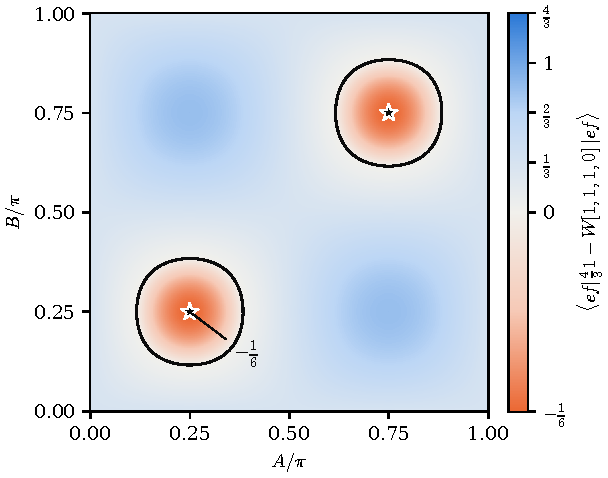
\includegraphics[width=0.58\textwidth]{fig_negative_region.pdf}
\caption{Expectation value of $\tfrac43\id-W[1,1,1,0]$ on the product vectors
$\ket e=\cos A\ket0+\sin A\ket2$, $\ket f=\cos B\ket0-\sin B\ket2$. The black curves
are the zero level; inside them the operator is negative on a separable state. The stars
mark the minimum $-1/6$, attained at $A=B=\pi/4$ (the vector \eqref{eq:psistar}) and at
$A=B=3\pi/4$.}
\label{fig:neg}
\end{figure}

\section{The exact separable bound in every dimension}\label{sec:exact}

\begin{theorem}[Decomposition certificate]\label{thm:cert}
Let $n\ge2$, $\alpha\in\mathbb{R}^n$, and let $v\in\mathbb{R}$, $\lambda\in[0,1]$ satisfy
\begin{equation}\label{eq:certcond}
v\ge\alpha_0+\lambda,\qquad v\ge\alpha_k,\qquad
(v-\alpha_k)(v-\alpha_{n-k})\ge(1-\lambda)^{2}\qquad(1\le k\le n-1).
\end{equation}
Then $v\,\id-W_\alpha=P+Q^{\G}$ with the positive semidefinite operators
\begin{align}
P&=n\lambda\,\ketbra{\phi^+}{\phi^+}+(v-\alpha_0-\lambda)\sum_i\ketbra{ii}{ii},\label{eq:P}\\
Q&=\sum_i\sum_{k=1}^{n-1}(v-\alpha_k)\ketbra{i,i+k}{i,i+k}
+(1-\lambda)\sum_{i\neq j}\ketbra{i,j}{j,i}.\label{eq:Q}
\end{align}
Consequently $v\,\id-W_\alpha$ is decomposable, hence block positive, and $\uW\le v$.
\end{theorem}

\begin{proof}
$P\ge0$ because $\lambda\ge0$ and $v-\alpha_0-\lambda\ge0$. The operator $Q$ vanishes on
the $n$ vectors $\ket{ii}$. The remaining $n^2-n$ basis vectors split into the
$n(n-1)/2$ unordered pairs $\{\ket{i,j},\ket{j,i}\}$, $i\neq j$, whose spans are mutually
orthogonal and invariant under $Q$. Hence $Q$ is the direct sum of a zero block and of
the $2\times2$ blocks
\begin{equation}\label{eq:block}
\begin{pmatrix}v-\alpha_k&1-\lambda\\[1pt]1-\lambda&v-\alpha_{n-k}\end{pmatrix},
\qquad k=j-i,
\end{equation}
because $\ket{j,i}=\ket{j,j+(n-k)}$ carries the weight $v-\alpha_{n-k}$. Each block is
positive semidefinite by \eqref{eq:certcond}; for $2k\equiv0$ the two diagonal entries
coincide and the condition reads $v-\alpha_k\ge1-\lambda$. Partial transposition leaves
the diagonal part of $Q$ unchanged and maps $\ketbra{i,j}{j,i}$ to $\ketbra{j,j}{i,i}$.
Hence $P+Q^{\G}$ has the entries $\lambda+(1-\lambda)=1$ on $\ketbra{ii}{jj}$,
$i\neq j$, the diagonal entries $\lambda+(v-\alpha_0-\lambda)=v-\alpha_0$ on $\ket{ii}$,
and $v-\alpha_k$ on $\ket{i,i+k}$, $k\neq0$. These are the entries of $v\,\id-W_\alpha$.
Finally $\bra{e,f}Q^{\G}\ket{e,f}=\bra{\bar e,f}Q\ket{\bar e,f}\ge0$.
\end{proof}

For $1\le k\le n/2$ define
\begin{equation}\label{eq:Bk}
B_k(\alpha)=\frac{(\alpha_0+1)^{2}-\alpha_k\alpha_{n-k}}{2(\alpha_0+1)-\alpha_k-\alpha_{n-k}}
\qquad\text{if}\quad \alpha_0+1>\max(\alpha_k,\alpha_{n-k}),
\end{equation}
and $B_k(\alpha)=-\infty$ otherwise. For even $n$ and $k=n/2$ this is
$B_{n/2}=\tfrac12(\alpha_0+\alpha_{n/2}+1)$.

\begin{theorem}[Exact separable bound]\label{thm:exact}
For all $n\ge2$ and all $\alpha\in\mathbb{R}^n$,
\begin{equation}\label{eq:L}
\uW=L_n(\alpha):=\max\bigl\{\alpha_0,\alpha_1,\dots,\alpha_{n-1},\,
B_1(\alpha),\dots,B_{\lfloor n/2\rfloor}(\alpha)\bigr\}.
\end{equation}
The maximum is attained on the following product vectors:
\begin{enumerate}
\item[(i)] basis vectors $\ket{i,i+k}$, with value $\alpha_k$;
\item[(ii)] two-level vectors
$(\sqrt t\,\ket i+\sqrt{1-t}\,\ket{i+k})\otimes(\sqrt{1-t}\,\ket i-\sqrt t\,\ket{i+k})$
with $1\le k\le n/2$ and $0\le t\le1$, with value
\begin{equation}\label{eq:gk}
g_k(t)=2(\alpha_0+1)\,t(1-t)+\alpha_k\,t^{2}+\alpha_{n-k}\,(1-t)^{2},
\end{equation}
whose maximum over $t$ equals $B_k(\alpha)$ if $\alpha_0+1>\max(\alpha_k,\alpha_{n-k})$
and $\max(\alpha_k,\alpha_{n-k})$ otherwise.
\end{enumerate}
Moreover $L_n(\alpha)\,\id-W_\alpha$ is decomposable.
\end{theorem}

\begin{proof}
\emph{Lower bound.} The values follow from Lemma~\ref{lem:prod}. In (i), $s_k=1$ and
$|\sum_ie_if_i|^2=\delta_{k0}$. In (ii), $s_0=2t(1-t)$, the weight $t^{2}$ lies on
$\ket{i,i+k}$ and the weight $(1-t)^{2}$ on $\ket{i+k,i}$, so $s_k=t^2$ and
$s_{n-k}=(1-t)^2$ if $2k\not\equiv0$ and $s_k=t^2+(1-t)^2$ if $2k\equiv0$, and
$\sum_ie_if_i=\sqrt{t(1-t)}-\sqrt{t(1-t)}=0$; this gives \eqref{eq:gk} in both cases. The
quadratic $g_k$ has $g_k(0)=\alpha_{n-k}$ and $g_k(1)=\alpha_k$. If
$\alpha_0+1>\max(\alpha_k,\alpha_{n-k})$ it is strictly concave with its maximum at
\begin{equation*}
t^{*}=\frac{\alpha_0+1-\alpha_{n-k}}{2(\alpha_0+1)-\alpha_k-\alpha_{n-k}}\in(0,1),
\qquad
g_k(t^{*})=\alpha_{n-k}+\frac{(\alpha_0+1-\alpha_{n-k})^{2}}{2(\alpha_0+1)-\alpha_k-\alpha_{n-k}}
=B_k(\alpha).
\end{equation*}
If $\alpha_0+1\le\max(\alpha_k,\alpha_{n-k})$, then
$g_k(t)\le\max(\alpha_k,\alpha_{n-k})\bigl(2t(1-t)+t^2+(1-t)^2\bigr)$ shows that the
maximum is attained at an endpoint and equals $\max(\alpha_k,\alpha_{n-k})$, which is
already covered by (i). Hence $\uW\ge L_n(\alpha)$.

\emph{Upper bound.} Write $L=L_n(\alpha)$ and apply Theorem~\ref{thm:cert} with $v=L$ and
$\lambda=\min(1,L-\alpha_0)$; then $\lambda\in[0,1]$ because $L\ge\alpha_0$. The first two
conditions in \eqref{eq:certcond} hold by the definition of $L$. If $\lambda=1$, the
third reads $(L-\alpha_k)(L-\alpha_{n-k})\ge0$ and holds. If $\lambda=L-\alpha_0<1$, the
third condition reads $(\alpha_0+1-L)^{2}\le(L-\alpha_k)(L-\alpha_{n-k})$, that is,
\begin{equation}\label{eq:fourth}
(\alpha_0+1)^{2}-\alpha_k\alpha_{n-k}\le L\,\bigl(2(\alpha_0+1)-\alpha_k-\alpha_{n-k}\bigr).
\end{equation}
In this case $\alpha_0+1>L\ge\max(\alpha_k,\alpha_{n-k})$, so $B_k$ is finite, the
factor on the right is positive, and \eqref{eq:fourth} is the inequality $L\ge B_k$ (for
$k>n/2$ use $B_{n-k}$, which is the same number). Hence $L\,\id-W_\alpha$ is decomposable
and $\uW\le L$.
\end{proof}

\begin{corollary}[No non-decomposable mirror]\label{cor:nogo}
Let $n\ge2$, $\alpha\in\mathbb{R}^n$, $W=W_\alpha$ and $\mu\in\mathbb{R}$. The following
are equivalent: (a) $\mu\id-W$ is block positive; (b) $\mu\ge L_n(\alpha)$; (c)
$\mu\id-W$ is decomposable. Hence the mirrored operator $\mu\id-W$ is
\begin{itemize}
\item not block positive, and so not a witness, for $\mu<L_n(\alpha)$;
\item a decomposable witness for $L_n(\alpha)\le\mu<\lmax(W)$;
\item positive semidefinite for $\mu\ge\lmax(W)$.
\end{itemize}
In no dimension is it a non-decomposable witness, and in no case does it detect a PPT
state. For this family the threshold of block positivity and the threshold of
decomposability coincide.
\end{corollary}

\begin{proof}
(a)$\Leftrightarrow$(b) is the definition of $\uW$ together with $\uW=L_n(\alpha)$. If
$\mu\ge L_n(\alpha)$, then $\mu\id-W=(\mu-L_n)\id+(L_n\id-W)$ is the sum of a positive
operator and a decomposable one, which gives (c), and (c) implies (a). The three cases
follow with \eqref{eq:lmax}.
\end{proof}

\begin{figure}[t]
\centering
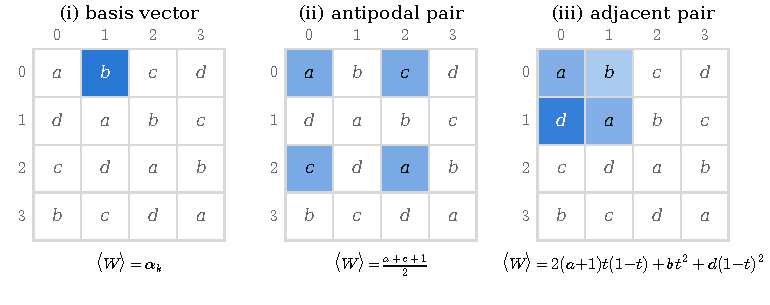
\includegraphics[width=0.95\textwidth]{fig_product_families.pdf}
\caption{The extremal product vectors of Theorem~\ref{thm:exact} for $n=4$, shown by
their weights $|e_i|^2|f_j|^2$ on the grid of basis vectors $\ket{i,j}$ (row $i$, column
$j$); each cell carries the diagonal coefficient of $W[a,b,c,d]$. Panel~(i) is a basis
vector; panels~(ii) and~(iii) are the two-level vectors with $k=2$ (antipodal levels,
$t=\tfrac12$) and $k=1$ (adjacent levels). The relative sign of the two components of
$f$ is chosen such that $\sum_ie_if_i=0$, which removes the negative term in
\eqref{eq:prodval}.}
\label{fig:fam}
\end{figure}

\begin{remark}[Low dimensions]\label{rem:low}
For $n=3$ there is one pair, $k=1$, and
\begin{equation}\label{eq:L3}
\uW=\max\Bigl\{a,\ b,\ c,\ \frac{(a+1)^{2}-bc}{2(a+1)-b-c}\Bigr\}
\qquad\text{for } W[a,b,c],
\end{equation}
the last term being present only if $a+1>\max(b,c)$. For $n=4$ there are the adjacent
pair $k=1$ and the antipodal pair $k=2$, and
\begin{equation}\label{eq:L4}
\uW=\max\Bigl\{a,\ b,\ c,\ d,\ \frac{a+c+1}{2},\ \frac{(a+1)^{2}-bd}{2(a+1)-b-d}\Bigr\}
\qquad\text{for } W[a,b,c,d],
\end{equation}
the last term being present only if $a+1>\max(b,d)$; the term $(a+c+1)/2$ may always be
kept, since it does not exceed $\max(a,c)$ when $a+1\le c$.
\end{remark}

\begin{remark}[Three versus four and more dimensions]\label{rem:fourthirds}
Consider the operator $W[1,\dots,1,0]$ with $\alpha=(1,1,\dots,1,0)$, which for $n=3$
is the Choi witness~\cite{Choi75,CKL92}. The pair $k=1$ contains the coefficient
$\alpha_{n-1}=0$ and gives $B_1=4/3$; every pair $2\le k\le n/2$ has
$\alpha_k=\alpha_{n-k}=1$ and gives $B_k=3/2$. Hence
\begin{equation}\label{eq:choi}
u_{W[1,1,0]}=\tfrac43\quad(n=3),\qquad u_{W[1,\dots,1,0]}=\tfrac32\quad\text{for every }n\ge4 .
\end{equation}
In dimension three only the pair $k=1$ exists, which is why the Choi witness has the
separable bound $4/3$. From dimension four on there are two-level product vectors whose
levels are not neighbours, and they raise the bound to $3/2$. The constant in
\eqref{eq:M43} is the three-dimensional value. We do not know how it was obtained; SBHCB
do not give a derivation.
\end{remark}

\begin{remark}[Relation to the conjecture on mirrors of optimal witnesses]\label{rem:conj}
Corollary~\ref{cor:nogo} establishes, for the whole family \eqref{eq:Walpha} in every
dimension, the dichotomy that~\cite{BBHC23} conjectured for mirrors of optimal witnesses:
the mirror is positive or a decomposable witness. No optimality assumption enters; the
statement holds for optimal and non-optimal witnesses and even for operators $W_\alpha$
that are not witnesses. The counterexample of~\cite{CBBH25} shows that the dichotomy
fails for other witnesses, so Corollary~\ref{cor:nogo} delimits a family in which it is a
theorem. For the three-dimensional family SBHCB~(71), which satisfies
$a+b+c=a^2+b^2+c^2=2$, formula \eqref{eq:L3} shows that the mirror at $\mu=\uW$ is
positive semidefinite if and only if $a\le1/3$ and a decomposable witness for $a>1/3$;
this is Proposition~6 of~\cite{SBHCB26}, which is thereby confirmed.
\end{remark}

\section{The two classes of the audited paper}\label{sec:classes}

SBHCB restrict the parameters of \eqref{eq:W4} by $a+b+c+d=a^2+b^2+c^2+d^2=3$, $ac+bd=1$
and $(a+c)(b+d)=2$ (SBHCB~(73)), which guarantees block positivity of $W$, and
distinguish two classes of solutions. With the parametrizations of SBHCB~(74) and (76)
they are
\begin{align}
\text{class I:}\quad& a=\tfrac12(2-\sin\theta),\ b=\tfrac12(1+\cos\theta),\ c=2-a,\ d=1-b,
&&\theta\in[0,2\pi),\label{eq:classI}\\
\text{class II:}\quad& a=\tfrac12(1+\cos\theta),\ b=\tfrac12(2-\sin\theta),\ c=1-a,\ d=2-b,
&&\theta\in[0,\pi].\label{eq:classII}
\end{align}
In SBHCB~(74) the last relation is printed as $d=\mu-b$; the constraints require $d=1-b$.
The witness $W[1,1,1,0]$ is the member $\theta=0$ of class~I. For $n=4$ the conditions
\eqref{eq:certcond} read $v\ge a+\lambda$, $v\ge c+1-\lambda$, $v\ge\max(b,d)$ and
$(v-b)(v-d)\ge(1-\lambda)^2$.

\begin{corollary}[Class I]\label{cor:classI}
For every $\theta$, the class-I witness $W_{\mathrm I}(\theta)$ has $\uW=3/2$, attained
on the antipodal vector \eqref{eq:psistar}, and
\begin{equation}\label{eq:decI}
\tfrac32\id-W_{\mathrm I}(\theta)=2(1+\sin\theta)\ketbra{\phi^+}{\phi^+}+Q_\theta^{\,\G},
\end{equation}
where $Q_\theta\ge0$ is the operator \eqref{eq:Q} with $v=\tfrac32$ and
$\lambda=\tfrac12(1+\sin\theta)$. The mirrored operator $\mu\id-W_{\mathrm I}(\theta)$ is
not block positive for $\mu<\tfrac32$, a decomposable witness for
$\tfrac32\le\mu<2-\tfrac12\sin\theta$, and positive semidefinite for
$\mu\ge2-\tfrac12\sin\theta$. In particular, no member of class~I has a non-decomposable
mirror. At $\mu=\tfrac32$ the mirror is positive semidefinite only for $\theta=\pi/2$.
\end{corollary}

\begin{proof}
$(a+c+1)/2=3/2$ for all $\theta$, so $\uW\ge3/2$. For the converse take $v=\tfrac32$ and
$\lambda=\tfrac12(1+\sin\theta)$ in Theorem~\ref{thm:cert}: then $a+\lambda=\tfrac32$,
$c+1-\lambda=\tfrac32$, $b,d\le1$, and
$(v-b)(v-d)=\tfrac14(4-\cos^2\theta)=\tfrac14(3+\sin^2\theta)\ge\tfrac14(1-\sin\theta)^2
=(1-\lambda)^2$. In \eqref{eq:P} the second term vanishes and $4\lambda=2(1+\sin\theta)$.
The three regimes follow from $\lmax(W)=a+1=2-\tfrac12\sin\theta$.
\end{proof}

For $\theta=0$ the decomposition \eqref{eq:decI} reads
\begin{equation}\label{eq:dec1110}
\begin{aligned}
\tfrac32\id-W[1,1,1,0]&=2\ketbra{\phi^+}{\phi^+}+Q_0^{\,\G},\\
Q_0&=\sum_i\Bigl[\tfrac12\ketbra{i,i+1}{i,i+1}+\tfrac12\ketbra{i,i+2}{i,i+2}
+\tfrac32\ketbra{i,i+3}{i,i+3}\Bigr]\\
&\quad+\tfrac12\sum_{i\neq j}\ketbra{i,j}{j,i},
\end{aligned}
\end{equation}
and $Q_0$ has the eigenvalues $0$, $1-\tfrac{1}{\sqrt2}$, $1$ and $1+\tfrac{1}{\sqrt2}$.
This identity, which can be checked by hand, proves at once that $3/2$ is the exact
separable maximum of $W[1,1,1,0]$ and that the corrected mirror is decomposable.

\begin{corollary}[Class II]\label{cor:classII}
For the class-II witness $W_{\mathrm{II}}(\theta)$ one has $\uW=3/2$ for
$\theta\in[0,\pi/2]$, attained on a two-level vector with adjacent levels, and
$\uW=d=\lmax(W)$ for $\theta\in[\pi/2,\pi]$. Accordingly, the mirror at $\mu=\uW$ is a
decomposable witness for $\theta\in[0,\pi/2)$ and positive semidefinite for
$\theta\in[\pi/2,\pi]$.
\end{corollary}

\begin{proof}
For $\theta\in[0,\pi/2)$ we have $a+1>d\ge b$, and a direct computation gives
$(a+1)^2-bd=\tfrac32(1+\cos\theta)$ and $2(a+1)-b-d=1+\cos\theta$, so $B_1=\tfrac32$. The
other candidates in \eqref{eq:L4} are $a,b,c\le1$, $d\le\tfrac32$ and $(a+c+1)/2=1$. For
$\theta\in[\pi/2,\pi]$ we have $d\ge a+1$, so $B_1=-\infty$ and $L_4=d$, which equals
$\lmax(W)$ by \eqref{eq:lmax}; at $\theta=\pi/2$ both descriptions give $\tfrac32$.
\end{proof}

Corollary~\ref{cor:classII} agrees with the statement of~\cite{SBHCB26} on class~II, that
the mirrored operators are positive semidefinite for $\theta\in(\pi/2,\pi)$ and
decomposable witnesses for $\theta\in(0,\pi/2)$. The complete picture for both classes is
shown in Fig.~\ref{fig:phase}.

\begin{figure}[t]
\centering
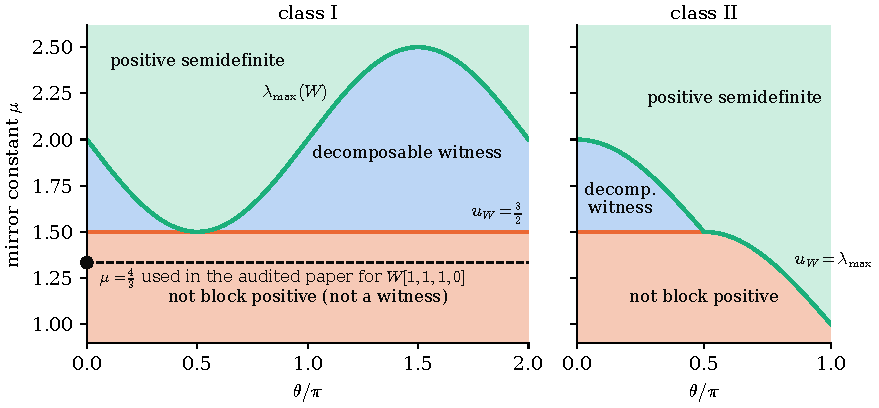
\includegraphics[width=0.95\textwidth]{fig_phase_diagram.pdf}
\caption{Nature of the mirrored operator $\mu\id-W$ for the two classes of $4\otimes4$
witnesses as a function of the mirror constant $\mu$. Below the separable bound $\uW$ the
operator is not block positive; between $\uW$ and $\lmax(W)$ it is a decomposable witness;
above $\lmax(W)$ it is positive semidefinite. A region of non-decomposable mirrors does
not exist (Corollary~\ref{cor:nogo}). The dot marks the operator \eqref{eq:M43}.}
\label{fig:phase}
\end{figure}

\section{Consequences for the audited paper and recomputation of its examples}\label{sec:sweep}

The main body of~\cite{SBHCB26}, in particular its multipartite constructions and its
$3\otimes3$ pair, is not called into question by what follows. The correction concerns
one example and the conclusion drawn from it.

\subsection{The \texorpdfstring{$4\otimes4$}{4x4} example}

\begin{enumerate}
\item The operator $M[1,1,1,0]=\tfrac43\id-W[1,1,1,0]$ is not an entanglement witness
(Section~\ref{sec:counter}). The mirrored operator of $W[1,1,1,0]$ is
$\tfrac32\id-W[1,1,1,0]$, and it is a decomposable witness with the decomposition
\eqref{eq:dec1110}.
\item For the PPT states $\rho_x$ of SBHCB~(75), which have the diagonal weights
$(3,x,1,1/x)$ on $\ket{i,i+k}$ and the entries $-1$ on $\ketbra{ii}{jj}$, we confirm the
value $\tr[(\tfrac43\id-W)\rho_x]=4(x^2-5x+4)/(3x)$ printed in~\cite{SBHCB26} (for the
unnormalized operator), which is negative for $x\in(1,4)$. With the correct constant,
\begin{equation}\label{eq:rhox}
\tr\bigl[(\tfrac32\id-W[1,1,1,0])\rho_x\bigr]=\frac{2(x^{2}-2x+3)}{x}
=\frac{2\bigl((x-1)^{2}+2\bigr)}{x}>0\qquad(x>0),
\end{equation}
as it must be for a decomposable operator. The states $\rho_x$ are not detected.
\item The conclusion that ``a pair of non-decomposable EWs can be mirrored with each
other'' is therefore not established by the $4\otimes4$ example, and by
Corollary~\ref{cor:classI} it cannot be established by any member of class~I, nor, by
Corollary~\ref{cor:nogo}, by any operator of the form \eqref{eq:Walpha}. The statement in
the introduction of~\cite{SBHCB26} that ``non-decomposable EWs can be a mirrored pair of
EWs while neither of them is optimal'' rests on this example and is left without support
by the paper; its $3\otimes3$ pair SBHCB~(77) consists of optimal witnesses.
\end{enumerate}

\subsection{Statements that are confirmed}

The following statements of~\cite{SBHCB26} were recomputed and found correct.
\begin{itemize}
\item \emph{Class I.} The witnesses are block positive; $W(\pi/2)=W[\tfrac12,\tfrac12,\tfrac32,\tfrac12]$
is decomposable (explicitly, $W(\pi/2)=2\ketbra{\chi}{\chi}+Q^{\G}$ with
$\ket\chi=\tfrac12\sum_i(-1)^i\ket{ii}$ and $Q\ge0$), and for the sampled values
$\theta\neq\pi/2$ the witness detects a PPT state.
\item \emph{Class II and the $3\otimes3$ family.} Proposition~6 and the classification of
the class-II mirrors, as discussed above.
\item \emph{The pair SBHCB~(77).} $W+M=4\,\id$; both operators are block positive
(numerical minimum over product vectors zero to $10^{-15}$); the states $\rho_W$ and
$\rho_M$ are PPT with $\tr(W\rho_W)=\tr(M\rho_M)=-\tfrac25$; and
$M=(U\otimes U^{*})W(U\otimes U^{*})^{\dagger}$ with the unitary of SBHCB~(78).
\item \emph{Three-qubit witnesses SBHCB~(60), (61).} $W+M=2\,\id$,
$M=Y^{\otimes3}WY^{\otimes3}$, $\|W\|=1+\sqrt{17}$, and non-negativity on product states,
for all eight sign choices. The states $\rho(x,y,z)$ and $\rho(b,c)$ are PPT across all
three cuts.
\item \emph{GHZ witnesses.} For $n=3,4$: $W_a+M_a=2^{1-n}\id$; the sum of the stabilizer
generators ranges over $[-(n-1),n-1]$ on product states; $M_a$ detects the state
SBHCB~(40).
\end{itemize}

\subsection{Minor inconsistencies}

The recomputation also brought up the following points. None of them affects a main
result of~\cite{SBHCB26}. Items 1--4 are definite and are corrected by the stated
replacement. Items 5 and 6 concern the detection of specific states; for these we report
what the printed definitions give, and we do not claim to know which of the printed
objects is the intended one. The computations behind items 5 and 6 are given in
Appendix~\ref{app:pauli}.
\begin{enumerate}
\item \emph{Section V.} The formula $\tr[W\rho_x]=a+bx+c+d/x-3$ is stated for
``$\rho_x$ in Eq.~(75)''. For that state the value is $3a+bx+c+d/x+3>0$. The formula
holds for the PPT state with diagonal weights $(1,x,1,1/x)$ and entries $+1$ on
$\ketbra{ii}{jj}$.
\item \emph{Normalization of mirrored pairs.} For the canonical and the two-measurement
GHZ witnesses the printed pairs do not satisfy $W+M=\mu\id$:
$\mu_c\id-W_c=\ketbra{GHZ_n}{GHZ_n}/(2^{n-1}-1)$ rather than $\ketbra{GHZ_n}{GHZ_n}$,
and $(2^n-2)W_{2m}+(2^n+2)M_{2m}=2\,\id$.
\item \emph{SBHCB~(49), (50).} Since the generators commute and take the values $\pm1$
independently, $\|W_a\|=2^{-n}(1+\tfrac{n}{n-1})=(2n-1)/((n-1)2^n)$, not
$n/((n-1)2^n)$; with SBHCB~(8) the corresponding tolerance is $1/(2(2n-1))$, not
$1/(2n)$. Tables~I and~II of~\cite{SBHCB26} give $1/(2n)$ and $1/(2n-1)$ for the same
witness up to a positive factor.
\item \emph{Local unitary below SBHCB~(40).} Conjugation by $Y$ on a set of qubits
multiplies $X^{\otimes n}$ by $(-1)^{\#Y}$. The operator
$\id\otimes Y\otimes\id\otimes Y\otimes\cdots$ therefore maps $W_a$ to $M_a$ if and only
if the number $\lfloor n/2\rfloor$ of factors $Y$ is odd; it fails for $n=4,5$. The
operator $Z\otimes Y\otimes\id\otimes Y$ works for $n=4$.
\item \emph{Label of the witness detecting $\rho(x,y,z)$.} With SBHCB~(60) as printed,
the value $2(x+y+z^{-1}-3)/\nu$ is $\tr[W[0,1,1]\rho(x,y,z)]$. For the label $W[0,1,0]$
used in the text and in Table~II one finds $2(x+y+z^{-1}+1)/\nu>0$.
\item \emph{The state $\rho(b,c)$.} With SBHCB~(60) and $\rho(b,c)$ as printed,
$\tr[W[1,1,0]\rho(b,c)]=2(c+7)/(b+c+6)>0$. None of the eight witnesses reproduces the
printed value $2(c-3)/(b+c+6)$; the smallest value over the eight labels is
$2(c-1)/(b+c+6)$, which is negative only for $c<1$.
\end{enumerate}

\section{Non-decomposable mirrored pairs outside the family}\label{sec:embed}

By Corollary~\ref{cor:nogo} a mirrored pair of non-decomposable witnesses cannot be found
among the operators \eqref{eq:Walpha} in any dimension. Such pairs exist in $3\otimes3$:
a pair of optimal non-decomposable witnesses was established in~\cite{CBBH25}, and
SBHCB~(77) presents such a pair. The following elementary construction carries any such
pair to all higher dimensions.

\begin{proposition}[Embedding]\label{prop:embed}
Let $W_3$ and $M_3$ be non-decomposable entanglement witnesses on
$\mathbb{C}^3\otimes\mathbb{C}^3$ with $W_3+M_3=\mu\,\id_9$, and let $\rho_W,\rho_M$ be PPT
states with $\tr(W_3\rho_W)<0$ and $\tr(M_3\rho_M)<0$. For $n\ge4$ let
$V:\mathbb{C}^3\to\mathbb{C}^n$ be the inclusion of the first three basis vectors,
$\Pi=VV^{\dagger}\otimes VV^{\dagger}$, and
\begin{equation}\label{eq:embed}
W_n=(V\otimes V)W_3(V\otimes V)^{\dagger}+\frac{\mu}{2}(\id-\Pi),\qquad
M_n=(V\otimes V)M_3(V\otimes V)^{\dagger}+\frac{\mu}{2}(\id-\Pi).
\end{equation}
Then $W_n+M_n=\mu\,\id_{n^2}$, and $W_n$ and $M_n$ are non-decomposable entanglement
witnesses on $\mathbb{C}^n\otimes\mathbb{C}^n$.
\end{proposition}

\begin{proof}
First, $\mu\ge0$: for any unit product vector,
$\mu=\bra{e,f}W_3\ket{e,f}+\bra{e,f}M_3\ket{e,f}\ge0$. The sum $W_n+M_n$ is
$\mu\Pi+\mu(\id-\Pi)$. For unit vectors $e,f\in\mathbb{C}^n$ let $e'=V^{\dagger}e$ and
$f'=V^{\dagger}f$, which need not be normalized. Then
\begin{equation*}
\bra{e,f}W_n\ket{e,f}=\bra{e',f'}W_3\ket{e',f'}+\frac{\mu}{2}\bigl(1-\|e'\|^2\|f'\|^2\bigr)\ge0 .
\end{equation*}
The first term is non-negative because block positivity is homogeneous and so holds for
unnormalized product vectors; the second because $\|e'\|,\|f'\|\le1$ and $\mu\ge0$. The
operator $(V\otimes V)\rho_W(V\otimes V)^{\dagger}$ is a normalized state, since
$V\otimes V$ is an isometry; it is PPT, since $V$ is real and partial transposition
commutes with the embedding; and its expectation value with $W_n$ equals
$\tr(W_3\rho_W)<0$. Hence $W_n$ is a witness that detects a PPT state. The same argument
applies to $M_n$.
\end{proof}

Applied to the pair SBHCB~(77), for which $\mu=4$ and
$\tr(W_3\rho_W)=\tr(M_3\rho_M)=-\tfrac25$, Proposition~\ref{prop:embed} yields a mirrored
pair of non-decomposable witnesses in $4\otimes4$ with $W_4+M_4=4\,\id_{16}$, each
detecting a PPT state with expectation value $-\tfrac25$, and likewise in every
$n\otimes n$. The existence of the three-dimensional pair is due to~\cite{CBBH25}; what
Proposition~\ref{prop:embed} adds is the passage to higher dimensions. The construction
is elementary, and we make no claim about optimality of $W_n$ and $M_n$. It shows that
the statement of~\cite{SBHCB26} about $4\otimes4$ is true as an existence statement,
although not for the example given there and, by Corollary~\ref{cor:nogo}, not within the
covariant family.

\section{Conclusion}

For the circulant covariant operators $W_\alpha$ on $\mathbb{C}^n\otimes\mathbb{C}^n$ the
maximum over product states is given by the closed formula \eqref{eq:L} in every
dimension. It is attained on product vectors supported on at most two levels, and the
matching upper bound comes from one explicit decomposition into a positive operator and a
partially transposed positive operator. The thresholds of block positivity and of
decomposability therefore coincide, and a non-decomposable mirror is impossible in this
family. The structure of the answer explains a dimensional effect: the set of two-level
supports grows with $n$, and levels that are not neighbours, which first appear for
$n=4$, can change the separable bound, as they do for the Choi-type witness, whose bound
jumps from $4/3$ to $3/2$.

Applied to~\cite{SBHCB26}, this shows that the mirrored operator given there for the
$4\otimes4$ witness $W[1,1,1,0]$ uses the three-dimensional constant $4/3$ in place of
$3/2$, that the corrected mirror is decomposable, and that the proposed PPT states are
not detected. A non-decomposable mirrored pair in $4\otimes4$ exists, but it has to be
sought outside the covariant family.

Two questions are left open. The operators \eqref{eq:Walpha} are the circulant members
of the larger class of $U\otimes U^{*}$-covariant operators of SBHCB~(67), in which the
diagonal weights need not be shift invariant; we do not know whether the two thresholds
still coincide there. And it is not known whether $4\otimes4$ admits a mirrored pair of
\emph{optimal} non-decomposable witnesses, as $3\otimes3$ does~\cite{CBBH25}.

\section*{Data and code availability}

The script \texttt{verify\_mirrored\_witnesses.py} reproduces every formula and numerical
statement of this paper (83 checks; it requires NumPy and SymPy and runs in about ninety
seconds; it was last run with Python~3.12, NumPy~1.26 and SymPy~1.13). The closed form
and the decomposition of Theorems~\ref{thm:cert} and~\ref{thm:exact} are tested for
$n=2,\dots,8$. The figures are generated by \texttt{make\_figures.py}. Both scripts, the
complete output of the verification run and the source of this manuscript are available
in the repository
\begin{center}
\url{https://github.com/Ruqing1963/seong-chruscinski-bae-2026-qst-audit}
\end{center}
\zenodonote

\section*{Declaration of generative AI and AI-assisted technologies in the manuscript preparation process}

The author (Ruqing Chen) conceived and directed this audit of the mathematical and
physical content of Ref.~\cite{SBHCB26}. Under the author's direction, the AI tools Claude
(Anthropic) and Gemini (Google) were used to assist with English academic writing,
\LaTeX{} typesetting, cross-checking of symbolic and algebraic derivations, and the
writing of the deterministic Python scripts \texttt{verify\_mirrored\_witnesses.py} and
\texttt{make\_figures.py}. All counterexamples, operator decompositions and proofs of
theorems were verified by deterministic programs and checked line by line by the author,
who takes full responsibility for the content of the publication.

\appendix
\section{Computations for the three-qubit states}\label{app:pauli}

SBHCB~(60) defines, with signs $\sigma_j=(-1)^{i_j}$ and
$\sigma_4=(-1)^{i_1+i_2+i_3+1}=-\sigma_1\sigma_2\sigma_3$,
\begin{equation*}
W[i_1,i_2,i_3]=\id-ZZZ-\sigma_1XXX-\sigma_2XYY-\sigma_3YXY-\sigma_4YYX .
\end{equation*}
The four operators $XXX$, $XYY$, $YXY$, $YYX$ have matrix elements only between a basis
vector $\ket{abc}$ and its complement, equal to $1$ for $XXX$ and to $-1$ or $+1$ for a
string with two $Y$ according to whether the two bits at the positions of the $Y$ are
equal or different.

\emph{The state $\rho(x,y,z)$.} It has the diagonal
$(1,x,y,z,z^{-1},y^{-1},x^{-1},1)/\nu$ and the single coherence $1/\nu$ between
$\ket{000}$ and $\ket{111}$. Then $\tr(ZZZ\rho)=(z-x-y+x^{-1}+y^{-1}-z^{-1})/\nu$,
$\tr(XXX\rho)=2/\nu$ and $\tr(XYY\rho)=\tr(YXY\rho)=\tr(YYX\rho)=-2/\nu$, so
\begin{equation*}
\nu\,\tr\bigl(W[i_1,i_2,i_3]\rho(x,y,z)\bigr)=2+2x+2y+2z^{-1}-2(\sigma_1-\sigma_2-\sigma_3-\sigma_4).
\end{equation*}
The bracket equals $4$ only for $(\sigma_1,\sigma_2,\sigma_3)=(1,-1,-1)$, the label
$[0,1,1]$, which gives $2(x+y+z^{-1}-3)$; for the label $[0,1,0]$ it equals $0$.

\emph{The state $\rho(b,c)$.} It has the diagonal $(1,1,1,b,c,1,1,1)/N$ with $N=6+b+c$
and the coherences $-1,-1,+1,-1$ (divided by $N$) on the pairs
$\{000,111\}$, $\{001,110\}$, $\{010,101\}$, $\{011,100\}$. Then $N\tr(ZZZ\rho)=b-c$,
$N\tr(XXX\rho)=-4$, $N\tr(XYY\rho)=4$, $N\tr(YXY\rho)=-4$ and $N\tr(YYX\rho)=4$, so
\begin{equation*}
N\,\tr\bigl(W[i_1,i_2,i_3]\rho(b,c)\bigr)=6+2c+4(\sigma_1-\sigma_2+\sigma_3-\sigma_4).
\end{equation*}
Under the constraint $\sigma_4=-\sigma_1\sigma_2\sigma_3$ the bracket takes only the
values $\pm2$, which gives $2c+14$ or $2c-2$. The printed value $2(c-3)$ would require
the bracket to equal $-3$.

\begin{thebibliography}{99}

\bibitem{SBHCB26} J.~Seong, A.~Bera, B.~C.~Hiesmayr, D.~Chru\'sci\'nski, and J.~Bae,
Mirrored entanglement witnesses for multipartite and high-dimensional quantum systems,
Quantum Sci.\ Technol.\ \textbf{11}, 015037 (2026); arXiv:2510.06863v2.

\bibitem{HHH96} M.~Horodecki, P.~Horodecki, and R.~Horodecki,
Separability of mixed states: necessary and sufficient conditions,
Phys.\ Lett.\ A \textbf{223}, 1 (1996).

\bibitem{Terhal00} B.~M.~Terhal, Bell inequalities and the separability criterion,
Phys.\ Lett.\ A \textbf{271}, 319 (2000).

\bibitem{LKCH00} M.~Lewenstein, B.~Kraus, J.~I.~Cirac, and P.~Horodecki,
Optimization of entanglement witnesses, Phys.\ Rev.\ A \textbf{62}, 052310 (2000).

\bibitem{GT09} O.~G\"uhne and G.~T\'oth, Entanglement detection,
Phys.\ Rep.\ \textbf{474}, 1 (2009).

\bibitem{CS14} D.~Chru\'sci\'nski and G.~Sarbicki,
Entanglement witnesses: construction, analysis and classification,
J.\ Phys.\ A: Math.\ Theor.\ \textbf{47}, 483001 (2014).

\bibitem{BCH20} J.~Bae, D.~Chru\'sci\'nski, and B.~C.~Hiesmayr,
Mirrored entanglement witnesses, npj Quantum Inf.\ \textbf{6}, 15 (2020).

\bibitem{Peres96} A.~Peres, Separability criterion for density matrices,
Phys.\ Rev.\ Lett.\ \textbf{77}, 1413 (1996).

\bibitem{BBHC23} A.~Bera, J.~Bae, B.~C.~Hiesmayr, and D.~Chru\'sci\'nski,
On the structure of mirrored operators obtained from optimal entanglement witnesses,
Sci.\ Rep.\ \textbf{13}, 10733 (2023).

\bibitem{CBBH25} D.~Chru\'sci\'nski, A.~Bera, J.~Bae, and B.~C.~Hiesmayr,
A mirrored pair of optimal non-decomposable entanglement witnesses for two qudits does
exist, Sci.\ Rep.\ \textbf{15}, 28205 (2025).

\bibitem{Choi75} M.-D.~Choi, Positive semidefinite biquadratic forms,
Linear Algebra Appl.\ \textbf{12}, 95 (1975).

\bibitem{CKL92} S.~J.~Cho, S.-H.~Kye, and S.~G.~Lee,
Generalized Choi maps in three-dimensional matrix algebra,
Linear Algebra Appl.\ \textbf{171}, 213 (1992).

\end{thebibliography}

\end{document}
